%
% 3
%
\section{Advanced data skills}

The following operations are \emph{not} covered in the course because they require extensive checks that would take too much time to process. You are strongly advised \emph{not} to try any of the operations below, unless you can allocate several additional working hours to your project in the first weeks of class.

% 3.1
%
\subsection{Weighting}

\newthought{An observation} is one single instance of the unit of analysis. The unit of analysis is a unique entity for which the data were collected, and can be virtually anything as long as a clear definition exists for it. Voters, countries or companies are common units of analysis, but events like natural disasters and civil wars are also potential candidates.

The definition of the unit of analysis sets the population from which to sample from. For instance, if you are studying voting behaviour in France, your study is likely to apply only to the French adult population that was allowed to vote at the time you conducted your research. Dataset codebooks usually discuss these issues at length.
The sample design then sets how observations were collected. The various techniques that apply to sampling form a crucial component of quantitative methods, that can be broken down to a few essential elements that you will need to understand in order to assess the representativeness of your data:
\begin{itemize}
 \item The \emph{sample size} designates the number of observations, noted $N$, contained in the dataset. Since variables often have missing values, large segments of your analysis might run on lower number of observations than $N$. 
 Sample size affects statistical significance through sampling error, which characterises the difference between a sample parameter, such as the average level of support for Barack Obama in a sample of $N$ respondents, and a population parameter, such as the actual average level of support for Barack Obama in the full population of U.S. voters (the size of which we might know, or not).
 
 The Central Limit Theorem (CLT) shows that repeated sample means are normally distributed around the population mean.
 
 Sampling error is calculated using the standard error, from which are derived confidence intervals for parameters such as the sample mean. The standard error decreases either with the level of confidence of an estimate, or with the square root of the sample size. Consequently, the law of large numbers applies: larger sample sizes will approach population parameters better and are preferable to obtain robust findings.

 \item The \emph{sampling strategy} designates the method used to collect the units contained within the sample (i.e. the dataset) from a larger universe of units, which can be a reference population such as adult residents in the United States or all nation-states worldwide at a given point in time.
 
 Sampling strategy has an impact on representativeness. Surveys often try to achieve simple random sampling to select observations from a population, using a method of data collection designed to assign each member of the population an equal probability of being selected, so that the results of the survey can be generalised to the population.
 
 Random or systematic sampling from particular strata or clusters of the population are among the methods used by researchers to approximate that type of representativeness. These methods can only approximate the whole universe of cases, as when a study ends up containing a higher proportion of old women than the true population actually does, which is why observations in a sample will be weighted in order to better match the sample with its population of reference.
 
 Other methods of data collection rely on nonprobability sampling. When the unit of analysis exists in a small universe, such as states or stock market companies, or when the study is aimed at a particular population, such as Internet users or voters, the sampling strategy targets specific units of analysis, with results that are not necessarily generalizable outside of the sample.
 
 The sampling strategy can correct for design effects such as clustering, systematic noncoverage and selection bias, all of which negatively affect the representativeness of the sample. Representativeness can be obtained through careful research design and weighted sampling. Stata handles complex survey design with several weights options passed to the \cmd{svyset} and \cmd{svy:} commands, both covered at length in the Stata documentation.
\end{itemize}

Important: Neither sample size nor sampling strategy will remove measurement errors that occur at earlier or later stages of data collection. Representativeness is only one aspect of survey design. On the one hand, it is technically possible to collect representative answers to very poorly written survey questions that will ultimately measure nothing. Ambiguously worded questions, for instance, will trigger unreliable answers that will cloud the results regardless of the statistical power and representativeness carried by the sample size and strategy. There is no statistical solution to the bias induced by question wording and order. On the other hand, coding and measurement errors can reduce the quality of the data in any sample: again, representativeness does not control for such issues. The \enquote{garbage in, garbage out} principle applies: poorly designed studies will always yield poor results, if any.

Let's give an example. Here, we look at the 2008 wave of the \ess (\textsc{ess}). It contains a design weight variable (cmd{dweight})to account for the fact that some categories of the population are over-represented in its sample. The table below was obtained by selecting a few observations from the study, using the \cmd{sample} command with the \cmd{count} option to draw a random subsample of 10 observations; the \cmd{list} command was then used to display the country of residence, gender and age of each respondent in this subsample, along with the design and population weights.

\begin{docspec}
  use data/ess2008 \\
  sample 10, count \\
  list cntry gndr agea dweight pweight
\end{docspec}

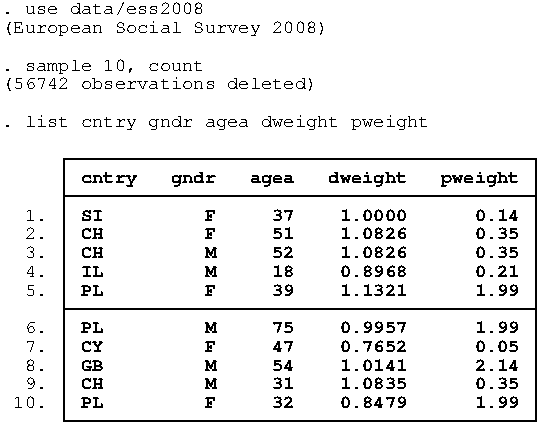
\includegraphics[width=250pt]{images/ess-sample.pdf}

The ESS documentation describes dweight (design weight) as follows:
\blockquote{Several of the sample designs used by countries participating in the ESS were not able to give all individuals in the population aged 15+ precisely the same chance of selection. Thus, for instance, the unweighted samples in some countries over- or under-represent people in certain types of address or household, such as those in larger households. The design weight corrects for these slightly different probabilities of selection, thereby making the sample more representative of a ‘true’ sample of individuals aged 15+ in each country.}
By looking at the subsample listed above, you can spot two observations for which the \cmd{dweight} variable is inferior to 1: both are females who were drawn from households that are over-represented by the sampling strategy used by the ESS, and are therefore assigned design weights under 1. Conversely, the other Russian female, aged 19, was drawn from a very under-represented household, and her assigned design weight is therefore above 2. These weights, when used with the \cmd{[weight]} operator or \cmd{svyset} command, ensure that these observations are given more or less importance when using frequencies and other aspects of the data, as to compensate for their under- or over-representation in the ESS sample in comparison to the actual population from which they were drawn.

The ESS documentation describes \cmd{pweight} (population weight) as follows:

\blockquote{This weight corrects for the fact that most countries taking part in the ESS have very similar sample sizes, no matter how large or small their population. Without weighting, any figures combining two or more country’s data would be incorrect, over-representing smaller countries at the expense of larger ones. So the Population size weight makes an adjustment to ensure that each country is represented in proportion to its population size.}

By looking again at the data above, you can indeed observe that the two respondents from Ukraine and Britain, two countries with large populations, have population weights around 2, and that the three respondents from Russia have an even higher population weight, whereas small countries like Cyprus or Switzerland have much smaller values. This makes sure that, when calculating the frequencies of a variable over several countries (such as the percentage of right-wing voters in Europe), the actual population size of each country is taken into account.

\newthought{In conclusion,} to weight the data at the European level, we need to account for both design and population weights. Design weights correct for the over- and under-representation of some socio-demographic groups, and population weights make sure that each national population accounts for its fraction of the overall European population.

This is done with the \cmd{svyset} command by creating a multiplication of both weights and using it as a probability weight:

\vskip 1em

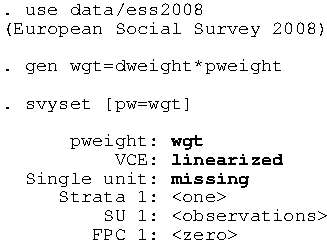
\includegraphics[width=150pt]{./images/ess-weight.pdf}

While population and design weights are pretty straightforward in this example, surveys can reach high levels of complexity when researchers try to capture multistage contexts by sampling from several strata and clusters of the target population. For example, large demographic surveys will often sample cities, and then sample neighbourhoods within them, and then sample households within them, and finally sample adults within them.

% 3.2
%
\subsection{Reshaping}

Time series data can come in two formats, depending on whether there is one row of observation per year (\enquote{wide} format) or several (\enquote{long} format). The \cmd{reshape} command can convert from one to the other format.
    
The course datasets are cross-sectional and do not require reshaping prior to analysis. Here are however some instructions in case you need to reshape a datafile. Let's suppose that the data are formatted with year values in columns, while the units of observation are displayed in rows. This format often applies to time series for country-level data.

Solving this issue requires to run a series of steps called \enquote{reshaping}. To reshape data for one variable, follow the following steps carefully:

\begin{itemize}
 \item Start by making sure that your data have been properly prepared: all variables must be numeric, and missing observations should be encoded as such.
 \item If your data is in a spreadsheet format (Excel, OpenOffice, CSV\dots), prepare your data as a CSV file. All variables should be labelled on the first line, and the rest of the file should contain only data (remove any other text or information). 
 \item Add a letter in front of each year. Select your first line, which contains the variable names, and then use the \enquote{Edit > Replace\dots} menu item in Excel to add a \enquote{y} in front of each year. For instance, if your data were collected for years 1960–2010, find \enquote{19} and replace by \enquote{y19}, and find \enquote{20} and replace by \enquote{y20}.
 \item Import using the \cmd{insheet} command, and check your data in the Stata data editor.
 \item Create a unique id value for each unit of observation (in this case, OECD countries) by typing \cmd{gen id = \_n} and then \cmd{order id}. This will add an additional variable to your data.
 \item To reshape your data, type \cmd{reshape long, y i(id) j(year)} to reshape your data columns that start with a \enquote{y}, for all rows identified by the \cmd{id} variable, into a different data format, called \enquote{long}, where the years will have been fit into a \cmd{year} variable.
 
\end{itemize}

Your dataset will have been converted from its initial \enquote{wide} format, with values for each year in columns, to a \enquote{long} format where the values for each year appear on separate rows.

Once you are in \enquote{long} mode, you can rename the variable that you were working on and drop the observations that you do not need (remember that you are working to obtain cross-sectional data and not time series).

\begin{docspec}
 ren y hexp \\
 la var hexp "Health expenditure per capita" \\
 drop if year != 1975 \\
\end{docspec}

If you are trying to reshape a dataset that is formatted in \enquote{wide} mode with more than one variable, more steps are required to separate the variables, as described in this tutorial: \url{http://dss.princeton.edu/training/DataPrep101.pdf} (locate the \enquote{Reshape} slides \#3–5).

Note that data reshaping will take a lot of time to achieve if you are merging and reshaping data over a large number of files. Do not try to merge more than a handful of datasets, as any other operation would require more time than this course can reasonably require from you.

Additional options in the \cmd{reshape} command allow to reshape data where the suffix is not numeric: type \cmd{help reshape} (or the shorthand version, \cmd{h reshape}) for additional documentation about this step.

% 3.3
%
% \subsection{Aggregation}

% - stratification over several levels of observation
% - nodes, ties, dyads
